
% !TEX encoding = UTF-8 Unicode 
% !TEX TS-program = xelatex

\documentclass[crop]{standalone}% 'crop' is the default for v1.0, before it was 'preview'
% xelatex -shell-escape -output-driver="xdvipdfmx -z 0" cover.tex
\usepackage{pdfx} 


\RequirePackage[usenames,dvipsnames]{xcolor}

\RequirePackage{tikz}
%\usetikzlibrary{...}% tikz package already loaded by 'tikz' option
 %  \usepackage[]{pdfx}
   \RequirePackage{fontspec}
    \RequirePackage[OT1]{fontenc}


    \RequirePackage{eulervm} % Must be before amssymb
    \RequirePackage{amsthm,amsmath}
    \RequirePackage{amssymb}

    % Check to see if this font is installed system-wide

    % Need bold font
    \setromanfont[Mapping=tex-text, Scale=0.95,AutoFakeSlant]{Trump Mediaeval LT Std}
    % Diacritics=Decompose not supported for this font
    % Hack:  accent \=a needed for Sankhya, not working with this font. Using  $\bar{\text{a}}$  	instead.
    % FIXME: ALSO Birkh\:{a}user broken

    % TODO: Change scale to 0.95?

    % Fix various accents that don't appear in this font.
    \DeclareTextAccent{\`}{EU1}{"0060}    %grave
    \DeclareTextAccent{\'}{EU1}{180}   %acute
    \DeclareTextAccent{\^}{EU1}{"02C6}   %circumflex
    \DeclareTextAccent{\~}{EU1}{"02DC}   %tilde
    \DeclareTextAccent{\"}{EU1}{168}   %dieresis
    \DeclareTextAccent{\H}{EU1}{"02DD}    %hungarumlaut
    \DeclareTextAccent{\r}{EU1}{"02DA}    %ring
    \DeclareTextAccent{\v}{EU1}{"02C7}    %caron
    \DeclareTextAccent{\u}{EU1}{"02D8}    %breve
    \DeclareTextAccent{\=}{EU1}{175}   %macron
    \DeclareTextAccent{\.}{EU1}{"02D9}    %dotaccent
    %
    % Hacks because font doesn't seem to support these accents
    \renewcommand{\v}[1]{$\check{\text{#1}}$}
    \renewcommand{\=}[1]{$\bar{\text{#1}}$}
    \renewcommand{\:}[1]{$\ddot{\text{#1}}$}

\begin{document}
\begin{tikzpicture}
\draw (0,0) -- (0,12in) -- (18in,12in) -- (18in,0in) -- (0,0);

\node[anchor=south west,inner sep=0] (image) at (0,0) {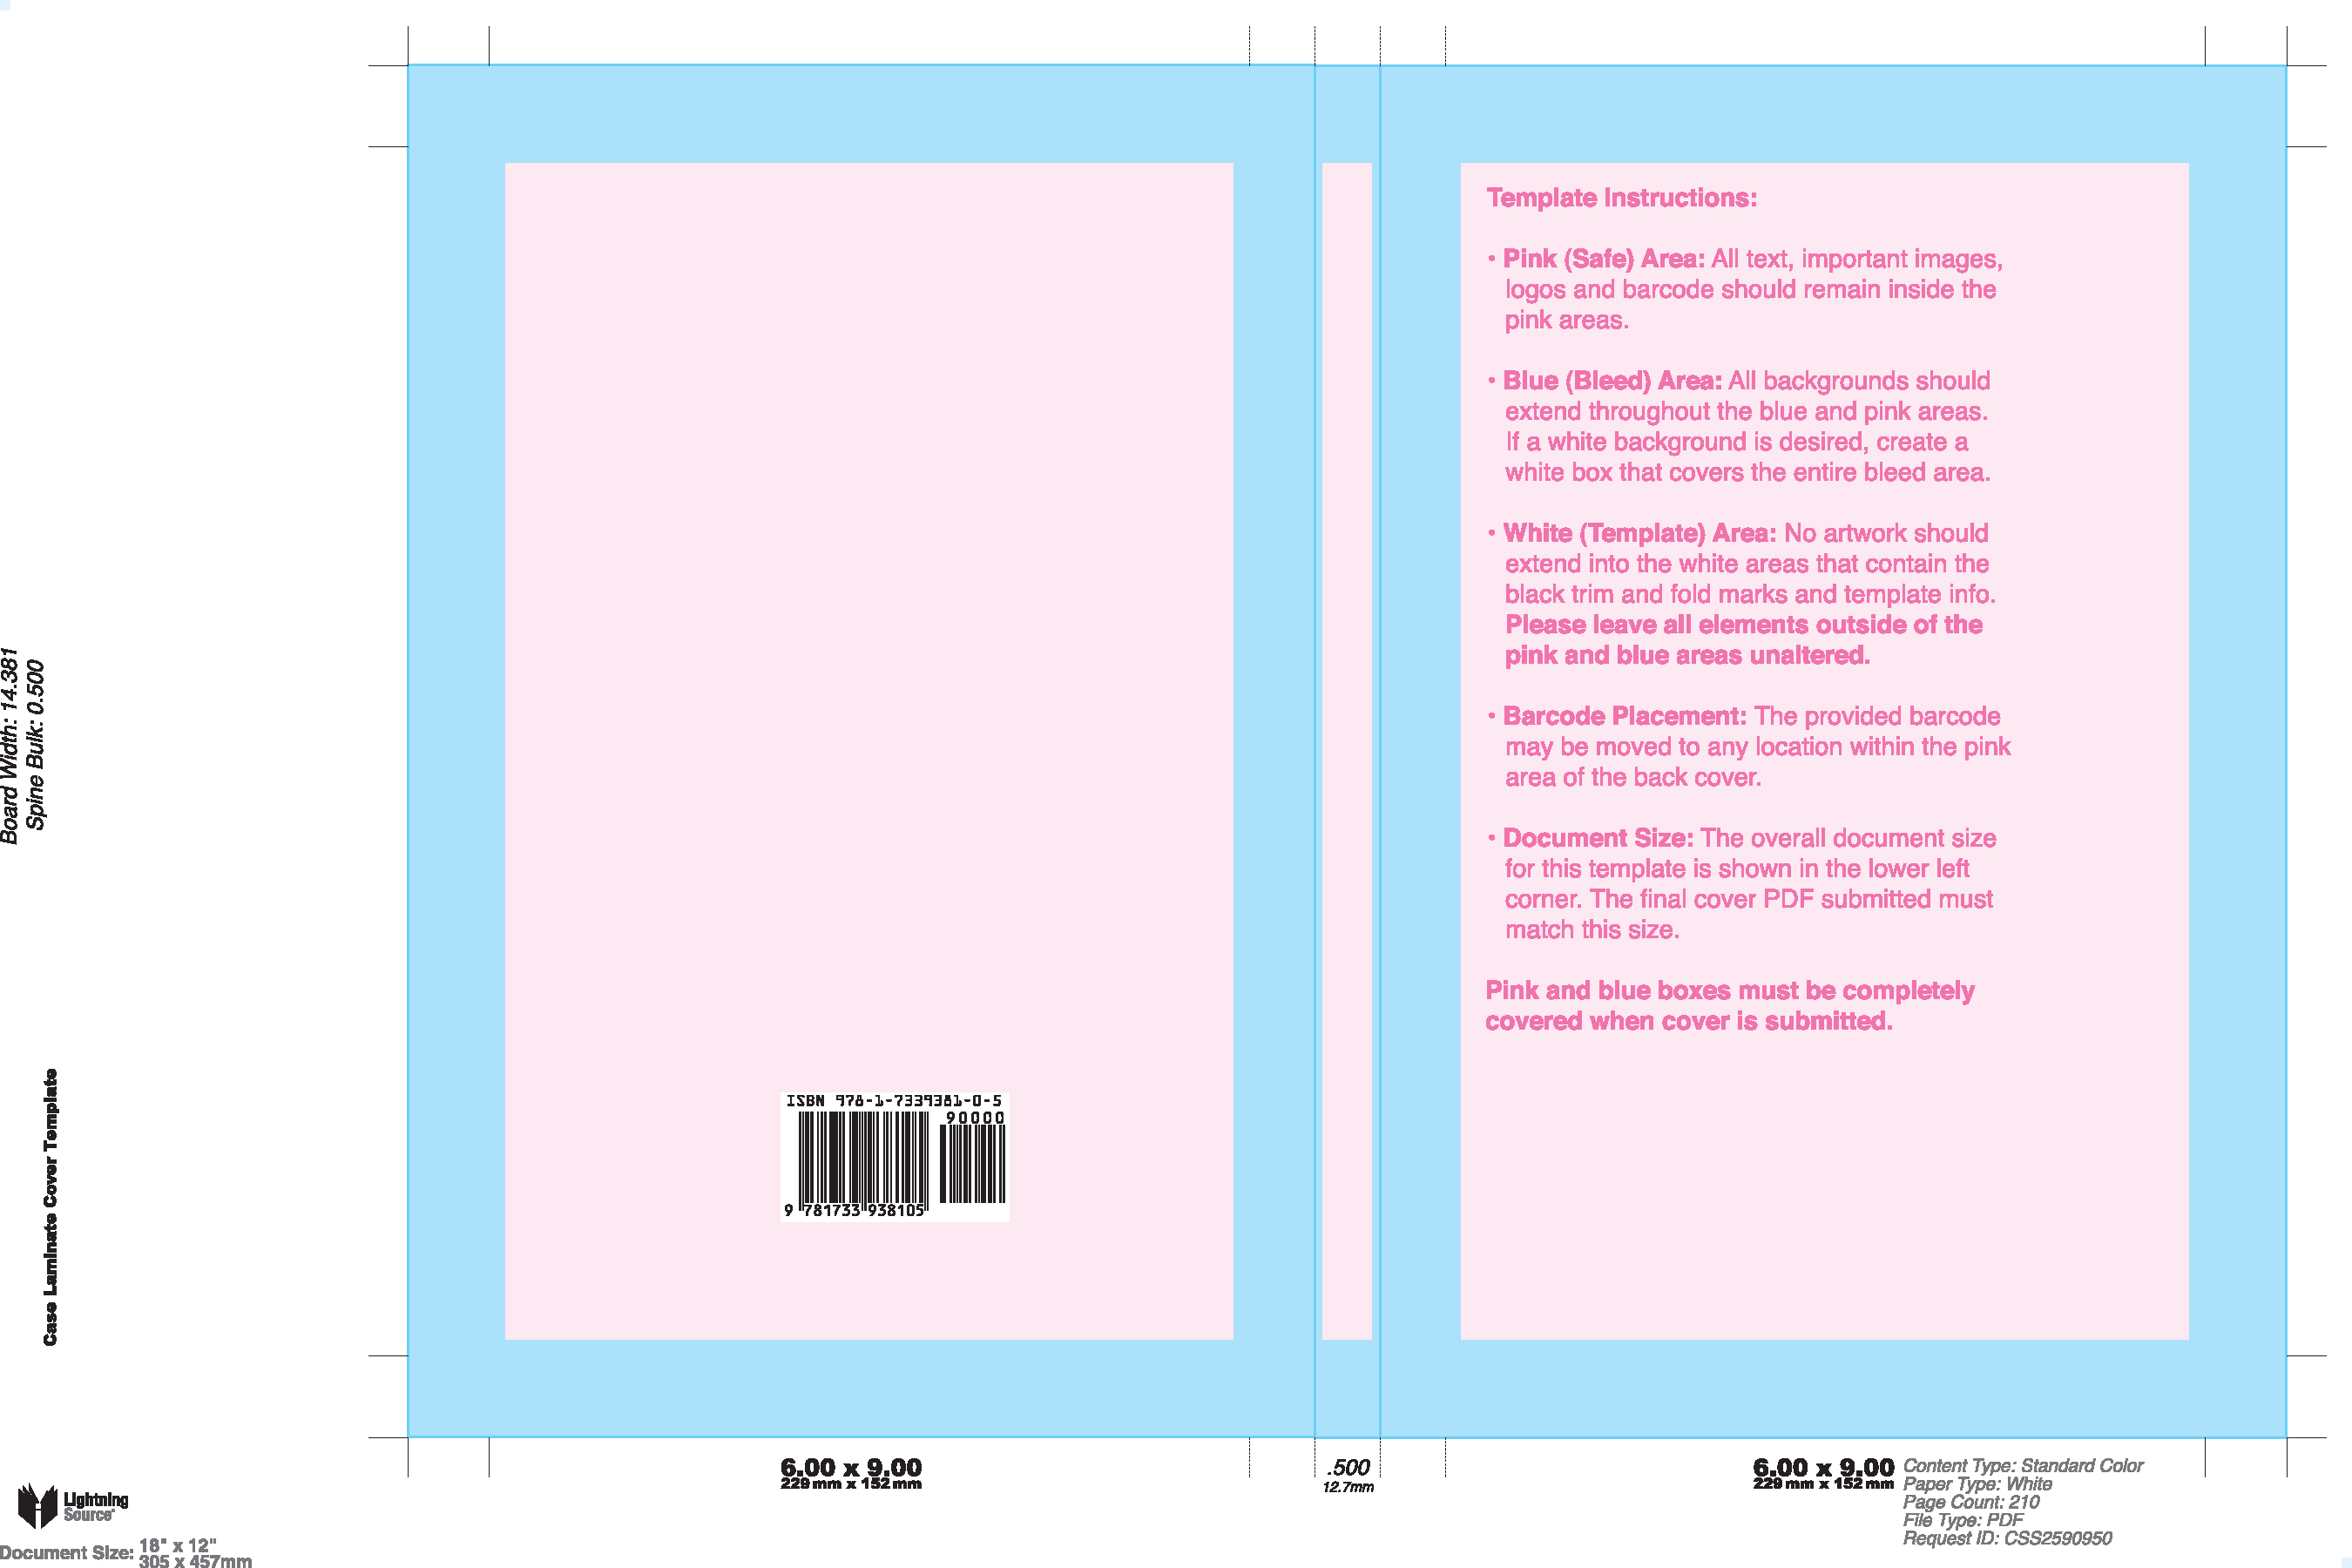
\includegraphics{9781733938105-Case.pdf}};

%\draw[help lines,step=1] (0,0) grid (47.5,30.5);
\draw[fill=gray, opacity=1.0] (7.95,2.55) -- (44.45,2.55) -- (44.45,29.25) -- (7.95,29.25) -- (7.95,2.55);

\node[rotate=-90, color=white] (title) at (26.2,15.75)  {\bf\LARGE\scshape Field Guide to Continuous Probability Distributions};
\node[rotate=-90, color=white] (title) at (26.2,25.6)  {\bf\LARGE\scshape G.E.~Crooks};
% \node[rotate=-90, color=white] (title) at (26.2,5.6)  {\bf\LARGE {\scshape BITS} };

%\node[anchor=south west,inner sep=0, opacity=1] (image) at (24.6,1.9) {\includegraphics{front.pdf}};
\node[anchor=south west,inner sep=0, opacity=1] (image) at (18.5,5) {
\includegraphics{isbn.pdf}};

\node[inner sep=0, opacity=1, scale=1.5] (image) at (35.5,10) {
\includegraphics{pdfCauchyNB.pdf}};

\node[color=white] (title) at (35.5,23)  {\bf \scshape{\huge Field Guide}};
\node[color=white] (title) at (35.5,21.75)  {\bf\scshape{\huge to}};
\node[color=white] (title) at (35.5,20.5)  {\bf\scshape{\huge Continuous}};
\node[color=white] (title) at (35.5,19.25)  {\bf\scshape{\huge Probability Distributions}};
\node[color=white] (title) at (35.5,17)  {\bf\scshape{\LARGE Gavin E. Crooks}};


\end{tikzpicture}


\end{document}






